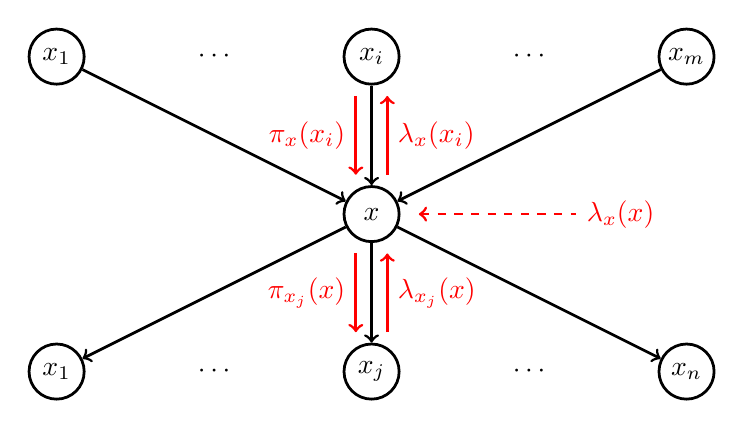
\begin{tikzpicture}[line width = 1pt,
                    node/.style = {draw, circle, inner sep = 0pt, minimum size = 0.7cm}]
    % Draw help lines.
    % \draw (0, 0) to[grid with coordinates]  (6, 8);
    
    \node[node] (cx1) at (0, 1) {$\cnode{x}_1$};
    \node             at (2, 1) {$\cdots$};
    \node[node] (cxj) at (4, 1) {$\cnode{x}_j$};
    \node             at (6, 1) {$\cdots$};
    \node[node] (cxn) at (8, 1) {$\cnode{x}_n$};

    \node[node] (px1) at (0, 5) {$\pnode{x}_1$};
    \node             at (2, 5) {$\cdots$};
    \node[node] (pxi) at (4, 5) {$\pnode{x}_i$};
    \node             at (6, 5) {$\cdots$};
    \node[node] (pxm) at (8, 5) {$\pnode{x}_m$};

    \node[node]   (x) at (4, 3) {$x$};
        
    \draw[->] (px1) -- (x);
    \draw[->] (pxi) -- (x);
    \draw[->] (pxm) -- (x);
    \draw[->] (x) -- (cx1);
    \draw[->] (x) -- (cxj);
    \draw[->] (x) -- (cxn);
    \pause

    \draw[->, red] (3.8, 4.5) -- (3.8, 3.5) node[anchor = east, midway, red] {$\pi_x(\pnode{x}_i)$};
    \pause

    \draw[->, red] (3.8, 2.5) -- (3.8, 1.5) node[anchor = east, midway, red] {$\pi_{\cnode{x}_j}(x)$};
    \pause
    
    \draw[->, red] (4.2, 1.5) -- (4.2, 2.5) node[anchor = west, midway, red] {$\lambda_{\cnode{x}_j}(x)$};
    \pause
    
    \draw[->, red] (4.2, 3.5) -- (4.2, 4.5) node[anchor = west, midway, red] {$\lambda_x(\pnode{x}_i)$};
    \pause    
    
    \draw[<-, dashed, red] (4.6, 3) -- ++(0:2cm) node[anchor = west, red] {$\lambda_x(x)$};
\end{tikzpicture}
